\chapter{Analisi della letteratura}
\label{cap:descrizione-stage}

\intro{Questo capitolo si pone l'obbiettivo di introdurre una conoscenza teorica per comprendere la scelta di utilizzare un algoritmo genetico per risolvere il problema in questione. Verranno esposti diversi metodi risolutivi, successivamente è presente una descrizione dei due approcci metaeuristici principali presi in considerazione e, infine, una spiegazione degli algoritmi evolutivi.}\\

\section{Approcci risolutivi}

Di seguito verranno descritti alcuni approcci per la risoluzione del problema di nesting.

\subsection{Approcci esatti}

Gli approcci esatti come la programmazione lineare intera mista (MILP) o i metodi di branch-and-bound hanno un costo computazionale elevato il che li rende difficilmente applicabili in contesti reali, dove spesso sono presenti un maggiore numero di vincoli specifici e le istanze possono essere di grandi dimensioni. La rappresentazione matematica diventa complessa quando si considerano problemi pratici che possiedono vincoli specifici.
Gilmore e Gomory (1961) hanno introdotto approcci lineari per il CSP\footcite{gilmore:linear-programming}.

\subsection{Approcci euristici e metaeuristici}

A differenza dei metodi esatti, le metaeuristiche consentono di affrontare istanze di problemi di grandi dimensioni fornendo soluzioni soddisfacenti in un tempo ragionevole, come afferma Talbi, «Gli algoritmi metaeuristici cercano buone soluzioni a problemi di ottimizzazione in circostanze in cui la complessità del problema affrontato o il tempo di ricerca disponibile non consentono l'uso di algoritmi di ottimizzazione esatti».\footcite{talbi:metaheuristics}

Gli algoritmi genetici (GA) che sono particolarmente efficaci per problemi combinatori complessi grazie alla capacità di esplorare grandi spazi di ricerca. I GA si sono dimostrati utili per il Nesting bidimensionale, permettendo l'evoluzione di soluzioni attraverso gli operatori di crossover e mutazione.

Jakobs (1996) ha introdotto uno dei primi GA per il problema di Nesting bidimensionale\footcite{jakobs:nesting}.

\subsection{Approcci ibridi}

Combinazioni di metaeuristiche e metodi esatti (ad esempio, utilizzo di euristiche per generare soluzioni iniziali per MILP) si dimostrano metodi risolutivi molto efficaci. L'uso di strategie ibride permette di bilanciare efficacia computazionale e qualità delle soluzioni, da un lato metodi euristici possono fornire informazioni utili ai metodi basati su programmazione lineare (es: soluzioni iniziali, upper bound). dall'altro lato metodi esatti possono essere inclusi in euristiche e metaeuristiche per risolvere sottoproblemi relativi a sottinsiemi di variabili. 

\section{Metaeuristiche}

La scelta di utilizzare una metaeuristica per il nostro problema è dovuta alla necessità di gestire vincoli pratici specifici per il caso Salvagnini, inoltre le metaeuristiche si prestano particolarmente alla massimizzazione dell'efficacia in tempi accettabili.

Le metaeuristiche sono tecniche di ottimizzazione che cercano di risolvere problemi complessi (spesso NP-hard) in modo approssimato, trovando soluzioni soddisfacenti anche quando metodi tradizionali come la programmazione matematica non sono applicabili a causa della difficoltà computazionale. Presentano diversi criteri, ognuno dei quali evidenzia le caratteristiche e le differenze tra le varie strategie di ottimizzazione:
\begin{itemize}
    \item Deterministici vs stocastici

    Deterministici: prendono decisioni completamente determinate (es.: ricerca locale, ricerca tabu). Utilizzando la stessa soluzione iniziale, il risultato finale sarà sempre lo stesso. \\
    Stocastici: introducono elementi di casualità (es.: simulated annealing, algoritmi evolutivi). La stessa soluzione iniziale può portare a risultati finali diversi. 
    \item Diversificazione vs intensificazione
    
    Diversificazione: si concentra sull'analisi di regioni inesplorate dello spazio di ricerca, per scoprire nuove aree potenzialmente promettenti.\\
    Intensificazione: si concentra sull'analisi approfondita delle regioni promettenti individuate tramite soluzioni accettabili, con l'obiettivo di trovare soluzioni migliori.
\end{itemize}

Le metaeuristiche vengono quindi classificate in due categorie principali: single solution-based e population-based. In generale, le metaeuristiche single solution-based sono orientate all'intensificazione mentre quelle population-based sono orientate alla diversificazione.
Vediamo le differenze in dettaglio.

\subsection{Single Solution-Based}

Le metaeuristiche single solution-based (o migliorative) operano partendo da una soluzione iniziale e cercando di migliorarla attraverso un processo iterativo. Ogni iterazione esplora il vicino della soluzione attuale, cercando di ottenere una soluzione migliore. Non vengono mai generate più soluzioni contemporaneamente, ma si cerca sempre di migliorare quella attuale. Le caratteristiche principali sono:
\begin{itemize}
    \item Soluzione unica: si lavora su una singola soluzione alla volta, cercando di modificarla attraverso diverse operazioni;
    \item Evoluzione locale: il processo di miglioramento della soluzione è locale, cioè si esplorano soluzioni vicine a quella attuale, dette vicinato.
\end{itemize}

Il scelta di un buon vicinato è uno degli aspetti fondamentali per le performance di un algoritmo migliorativo sia in termini di efficacia che di efficienza, come afferma Talbi, «Nel progettare una metaeuristica migliorativa, si incontra spesso un compromesso tra la dimensione (o diametro) e la qualità del vicinato da utilizzare e la complessità computazionale necessaria per esplorarlo. Progettare vicinati di grandi dimensioni può migliorare la qualità delle soluzioni ottenute, poiché vengono considerati più vicini a ogni iterazione (Figura 3.1) [...]. Tuttavia, ciò richiede un tempo computazionale aggiuntivo per generare e valutare un vicinato ampio».\footcite{talbi:ssb}
\begin{figure}[!ht] 
    \centering 
    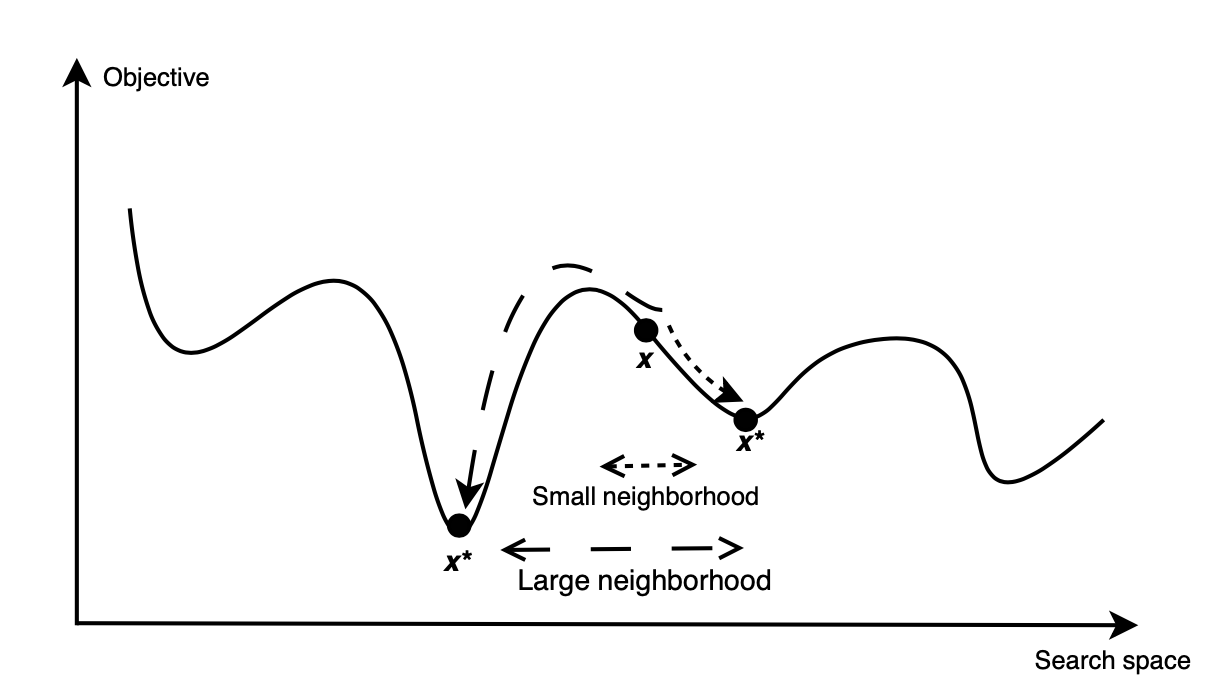
\includegraphics[width=0.9\columnwidth]{tesi/vicini} 
    \caption{Esempio di evoluzione della soluzione x, nello spazio di ricerca, con due dimenzioni di vicinato diverse}
\end{figure}

Anche con la di un vicinato adeguato, occorre tenere in considerazione due possibili criticità:
\begin{itemize}
    \item Rischio di ottimizzazione locale: poiché esplorano solo soluzioni vicine a quella attuale, c'è il rischio di rimanere bloccati in un minimo locale (local optima) senza riuscire a trovare la soluzione globale ottima (global optima) (Figura 3.2);
    \item Esplorazione limitata: spesso non sono in grado di esplorare efficacemente spazi di soluzioni vasti o complessi.
\end{itemize}

\begin{figure}[!ht] 
    \centering 
    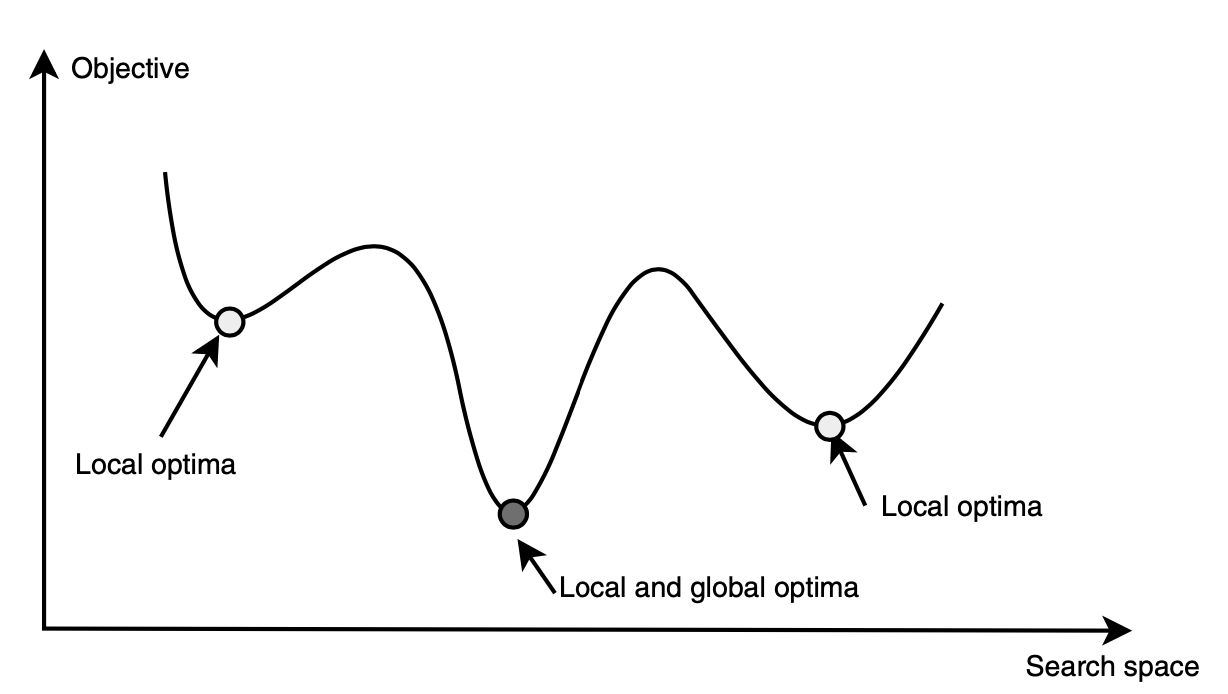
\includegraphics[width=0.9\columnwidth]{tesi/ottimi} 
    \caption{Minimi locali e minimi globali in uno spazio di ricerca, possono esserci più minimi globali}
\end{figure}

\subsection{Population-Based}

Le metaeuristiche population-based possono essere viste come un miglioramento iterativo di una popolazione di soluzioni. In primo luogo, la popolazione viene inizializzata. Successivamente, viene generata una nuova popolazione di soluzioni. Infine, questa nuova popolazione viene integrata in quella attuale utilizzando alcune procedure di selezione (Figura 3.3). Il processo di ricerca si interrompe quando viene soddisfatta una determinata condizione (criterio di arresto). %[talbi pagina 190] 
Le caratteristiche principali sono:
\begin{itemize}
    \item Soluzioni multiple: l'algoritmo opera su una popolazione di soluzioni che vengono evolute nel tempo;
    \item Evoluzione globale: la popolazione viene aggiornata in modo che le soluzioni migliori vengano selezionate per creare nuove soluzioni, combinando diversità e convergenza.
\end{itemize}

\begin{figure}[!ht] 
    \centering 
    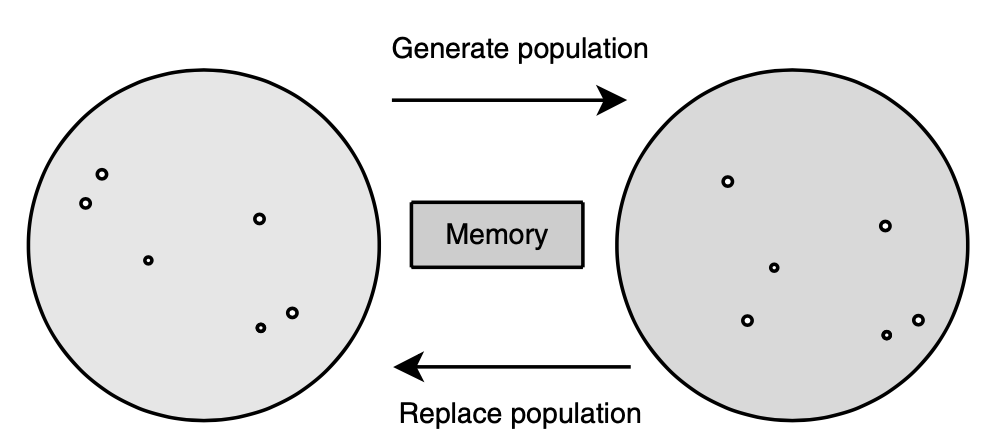
\includegraphics[width=0.9\columnwidth]{tesi/popolazione} 
    \caption{Principio generale delle metaeuristiche population-based}
\end{figure}

Grazie alla combinazione fra soluzioni multiple e evoluzione globale, mantenendo le soluzioni migliori di una data popolazione, le metaeuristiche population-based bilanciano la diversificazione (cercare nuove aree dello spazio delle soluzioni) e l'intensificazione (migliorare le soluzioni trovate). In particolare, la diversificazione aumenta la possibilità di evitare minimi locali, poiché operano su spazi di ricerca vasti, e le soluzioni della popolazione possono convergere verso la soluzione globale grazie all'intensificazione generata dal mantenere le soluzioni migliori iterazione dopo iterazione.

Come vedremmo nel capitolo 6, il punto centrale durante la fase di test dell'algoritmo è la parametrizzazione, infatti, l'ottimizzazione dei parametri della popolazione (come la dimensione della popolazione e i tassi di crossover e mutazione) può essere complessa e richiedere diversi tentativi per evitare il rischio di over-tuning, ovvero adattare i parametri a solo certe istanze con determinate caratteristiche.

\subsection{Confronto single solution-based e population-based}

\begin{table}[!ht]
    \centering
    \renewcommand{\arraystretch}{1.7}
    \begin{tabular}{|>{\raggedright\arraybackslash}p{4cm}|>{\raggedright\arraybackslash}p{4cm}|>{\raggedright\arraybackslash}p{4cm}|}
    \hline
    \textbf{Caratteristica} & \textbf{Single Solution-Based} & \textbf{Population-Based} \\ \hline
    Numero di soluzioni esplorate & Una sola soluzione alla volta & Più soluzioni contemporaneamente \\ \hline
    Esplorazione dello spazio di ricerca & Localizzata, vicina alla soluzione attuale, focus su intensidicazione & Maggiore esplorazione e diversificazione \\ \hline
    Rischio di ottimizzazione locale & Più alto, poiché esplora soluzioni vicine & Più basso, grazie alla diversità della popolazione \\ \hline
    Costo computazionale & Generalmente più efficiente & Più costoso a causa della popolazione di soluzioni \\ \hline
    \end{tabular}
    \caption{Confronto tra metaeuristiche single solution-based e population-based.}
    \label{tab:comparison}
\end{table}

In conclusione le single solution-based si focalizzano su una sola soluzione e migliorano gradualmente questa soluzione attraverso piccole modifiche, tuttavia, rischiano di restare bloccate in ottimi locali. Le population-based lavorano con una popolazione di soluzioni, permettendo una migliore esplorazione dello spazio di ricerca e riducendo il rischio di ottimizzazione locale, ma tendenzialmente con un costo computazionale maggiore (Tabella 3.1).

Scegliamo di sviluppare un algoritmo popilation-based dato si teme che la beam search, essendo una single solution-based, possa bloccarsi in dei minimi locali. Nel seguente paragrafo introduciamo alcuni tipi di metaeuristiche popilation-based per poter scegliere quella più adatta.

\section{Algoritmi evolutivi}

Nel XIX secolo, i principi dell'ereditarietà di J. Mendel e la teoria dell'evoluzione di C. Darwin (1859) hanno gettato le basi per lo sviluppo, negli anni '80 del Novecento, degli algoritmi evolutivi (EA). Questi metodi computazionali traggono ispirazione dai processi evolutivi naturali per risolvere problemi complessi di ottimizzazione. Tra i principali paradigmi sviluppati sono presenti gli algoritmi genetici (Holland), le strategie evolutive (Rechenberg, Schwefel), la programmazione evolutiva (Fogel) e la programmazione genetica (Koza). Sebbene ciascun approccio presenti peculiarità, tutti condividono il principio di evoluzione di una popolazione attraverso iterazioni basate su selezione, riproduzione e variazione.

Gli EA si basano sul concetto di competizione. Rappresentano una classe di algoritmi di ottimizzazione iterativi che simulano l'evoluzione delle specie (Figura 3.4). Si basano sull'evoluzione di una popolazione di individui, solitamente generata in modo casuale, e ogni individuo nella popolazione rappresenta una versione codificata di una soluzione provvisoria. Una funzione obiettivo associa a ogni individuo un valore di fitness che indica la sua idoneità al problema. A ogni passo, vengono selezionati gli individui che formeranno i genitori, seguendo un paradigma di selezione in cui gli individui con un valore di fitness migliore hanno una maggiore probabilità di essere scelti. Successivamente, gli individui selezionati vengono riprodotti utilizzando operatori di variazione (ad esempio, crossover e mutazione) per generare nuovi discendenti. Infine, viene applicato uno schema di sostituzione per determinare quali individui della popolazione sopravvivranno tra i discendenti e i genitori. Questa iterazione rappresenta una generazione (Figura 3.4). Questo processo viene ripetuto fino a quando non si verifica un criterio di arresto. [talbi pagina 199]

\begin{figure}[!ht] 
    \centering 
    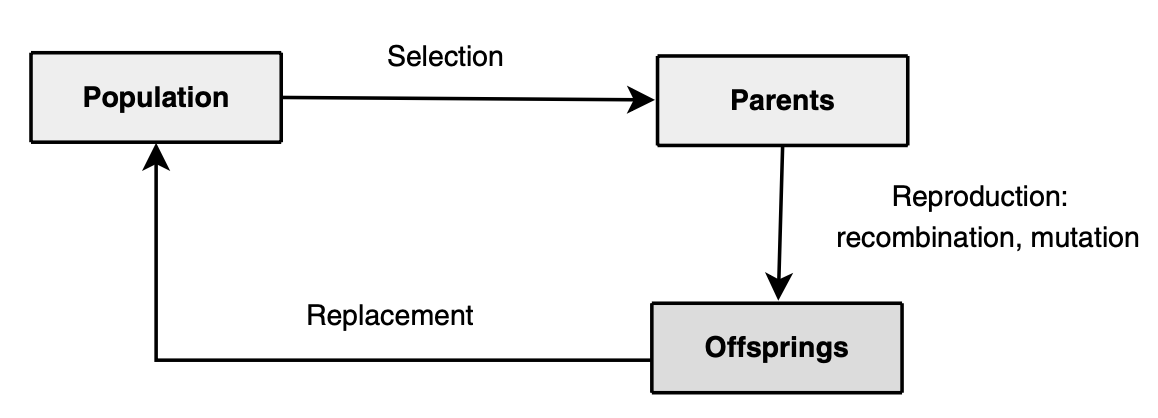
\includegraphics[width=0.9\columnwidth]{tesi/evoluzione} 
    \caption{Una generazione negli algoritmi evolutivi}
\end{figure}

Negli algoritmi evolutivi, il genotipo rappresenta la codifica, mentre il fenotipo rappresenta la soluzione. Pertanto, il genotipo deve essere decodificato per generare il fenotipo. Gli operatori di variazione agiscono a livello di genotipo, mentre la funzione di fitness utilizza il fenotipo dell'individuo associato (Figura 3.5). La fitness di un individuo è un valore calcolato per misurare quanto quella soluzione sia adatta al problema. 

\begin{figure}[!ht] 
    \centering 
    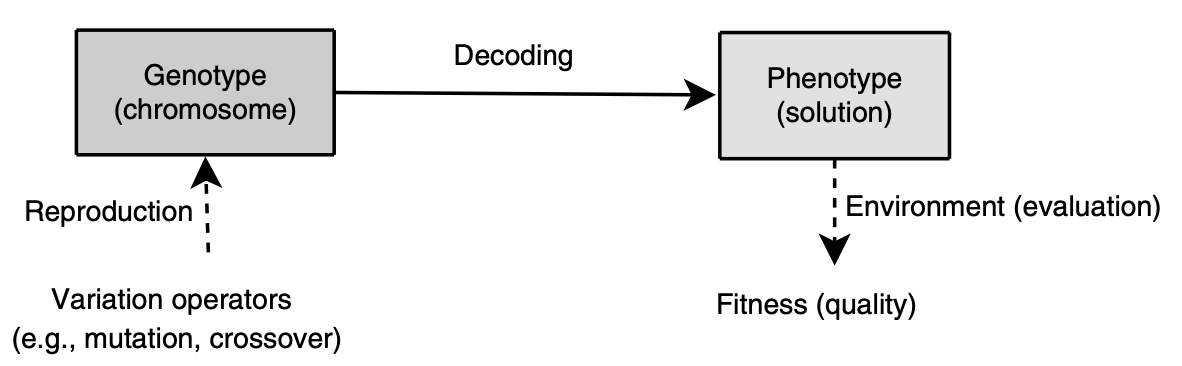
\includegraphics[width=0.9\columnwidth]{tesi/decoding} 
    \caption{Genotipo e fenotipo negli algoritmi evolutivi}
\end{figure}

Nelle sezioni seguenti verranno evidenziate le principali differenze tra le varie famiglie di algoritmi evolutivi. Successivamente, l'attenzione sarà focalizzata sui loro componenti di ricerca comuni.

\subsection{Algoritmi genetici}

Gli algoritmi genetici (Genetic Algorithms - GA) rappresentano una classe molto popolare di algoritmi evolutivi. Tradizionalmente, i GA sono associati all'uso di una rappresentazione binaria, ma oggi è possibile trovare GA che utilizzano altri tipi di rappresentazioni. Un GA applica solitamente un operatore di crossover a due soluzioni, che svolge un ruolo fondamentale, oltre a un operatore di mutazione che modifica casualmente i contenuti dell'individuo per promuovere la diversificazione delle soluzioni. I GA utilizzano una selezione probabilistica che originariamente è la selezione proporzionale. La sostituzione è generazionale, il che significa che i genitori vengono sistematicamente sostituiti dai discendenti. L'operatore di crossover si basa sul crossover a n punti o uniforme, mentre la mutazione consiste nel flipping di bit. Una probabilità fissa pm (rispettivamente pc) viene applicata all'operatore di mutazione (rispettivamente crossover).

\subsection{Strategie evolutive}

Le strategie evolutive (evolution strategies - ES) sono prevalentemente applicate all'ottimizzazione continua, dove le rappresentazioni si basano su vettori di valori reali.

Le ES utilizzano solitamente una sostituzione elitaria e una mutazione specifica distribuita normalmente (Gaussiana). Il crossover è raramente utilizzato. Nelle ES si distingue tra la popolazione dei genitori, di dimensione fissa, e la popolazione dei discendenti, di dimensione maggiore o uguale alla popolazione dei genitori. 

L'operatore di selezione è deterministico e si basa sul ranking della fitness. Pertanto, la parametrizzazione delle ES è altamente personalizzabile. La ricombinazione può essere discreta (simile al crossover uniforme dei GA) o intermedia (crossover aritmetico). Il loro principale vantaggio è l'efficienza in termini di complessità temporale.

\subsection{Programmazione evolutiva}

La programmazione evolutiva (evolutionary programming - EP) si concentra principalmente sulla mutazione e non utilizza la ricombinazione. Gli EP tradizionali sono stati sviluppati per far evolvere automi a stati finiti. Gli EP contemporanei sono stati successivamente applicati alla risoluzione di problemi di ottimizzazione continua utilizzando rappresentazioni a valori reali.

Utilizzano mutazioni distribuite normalmente e il principio di auto-adattamento dei parametri, come nelle ES. Il meccanismo di selezione dei genitori è deterministico, mentre il processo di selezione dei sopravvissuti (sostituzione) è probabilistico e si basa su un "torneo" stocastico di selezione.

La EP è meno utilizzata rispetto alle altre famiglie di algoritmi evolutivi, a causa della sua somiglianza con le ES.

\subsection{Programmazione genetica}

La programmazione genetica (genetic programming - GP) è un approccio evolutivo più recente la cui principale differenza rispetto alle altre famiglie evolutive è che gli individui evoluti sono essi stessi programmi (rappresentazione non lineare basata su alberi) anziché stringhe di lunghezza fissa provenienti da un alfabeto limitato di simboli (rappresentazione lineare). Questi programmi si evolvono combinandosi, riproducendosi o mutando, per dar luogo ad altri programmi che si adattano meglio a risolvere un determinato problema.

Le GP richiedono una popolazione molto grande (ad esempio, migliaia di individui), rendendole quindi molto costose dal punto di vista computazionale. La teoria della GP è meno sviluppata rispetto alle strategie evolutive e agli algoritmi genetici. Le GP contemporanee sono ampiamente utilizzate in compiti di apprendimento automatico e data mining, come la previsione e la classificazione.

\section{Gap di ricerca}

La letteratura fornisce una base solida per affrontare problemi di Nesting, ma il caso specifico Salvagnini presenta alcune lacune:

\begin{itemize}
    \item Approcci che integrano vincoli geometrici con vincoli di precedenza sono rari:
    \item Tecniche specifiche per il taglio comune e margini di punzonatura sono poco esplorate:
    \item L'uso di GA per istanze con vincoli multipli richiede ulteriori adattamenti, come operatori personalizzati.
\end{itemize}

Questi aspetti rappresentano opportunità per contribuire alla ricerca esistente sviluppando un algoritmo genetico mirato per il contesto descritto.